\chapter{Pruebas}

\section{Pruebas unitarias}

\begin{figure}[!ht]
	\begin{center}
		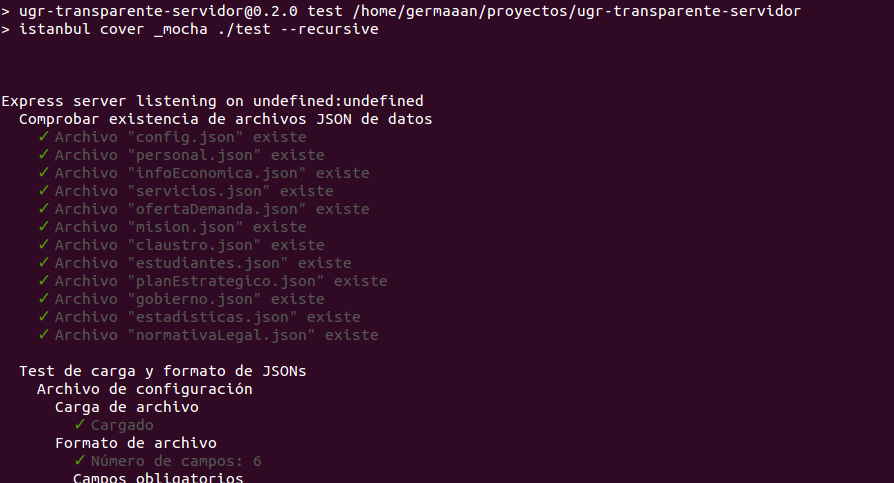
\includegraphics[width=1\textwidth]{../images/tests_unitarios_01.png}
		\caption{}
		\label{fig:tests_unitarios_01}
	\end{center}
\end{figure}

\begin{figure}[!ht]
	\begin{center}
		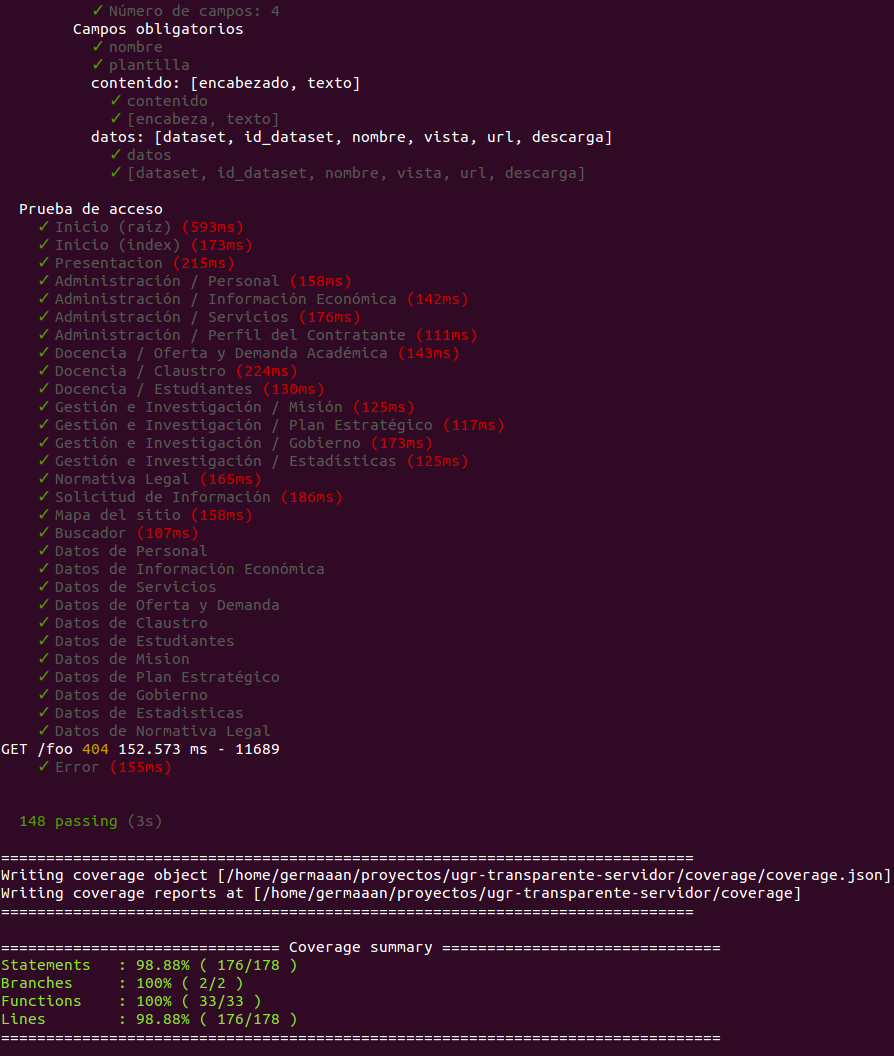
\includegraphics[width=1\textwidth]{../images/tests_unitarios_02.png}
		\caption{}
		\label{fig:tests_unitarios_02}
	\end{center}
\end{figure}

\section{Prueba de cobertura}

\begin{figure}[!ht]
	\begin{center}
		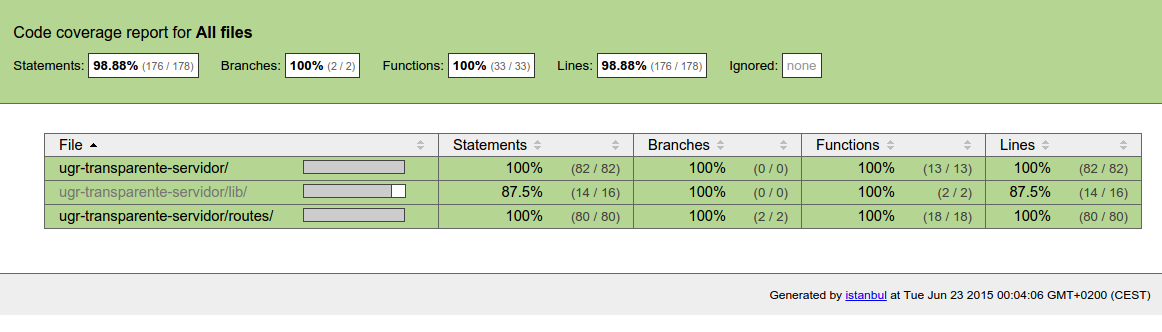
\includegraphics[width=1\textwidth]{../images/test_cobertura_01.png}
		\caption{}
		\label{fig:test_cobertura_01}
	\end{center}
\end{figure}

\begin{figure}[!ht]
	\begin{center}
		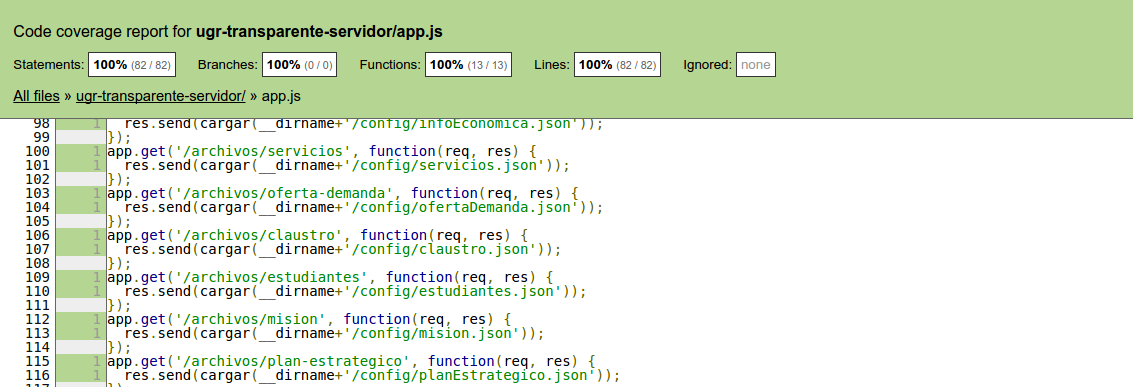
\includegraphics[width=1\textwidth]{../images/test_cobertura_02.png}
		\caption{}
		\label{fig:test_cobertura_02}
	\end{center}
\end{figure}

\begin{figure}[!ht]
	\begin{center}
		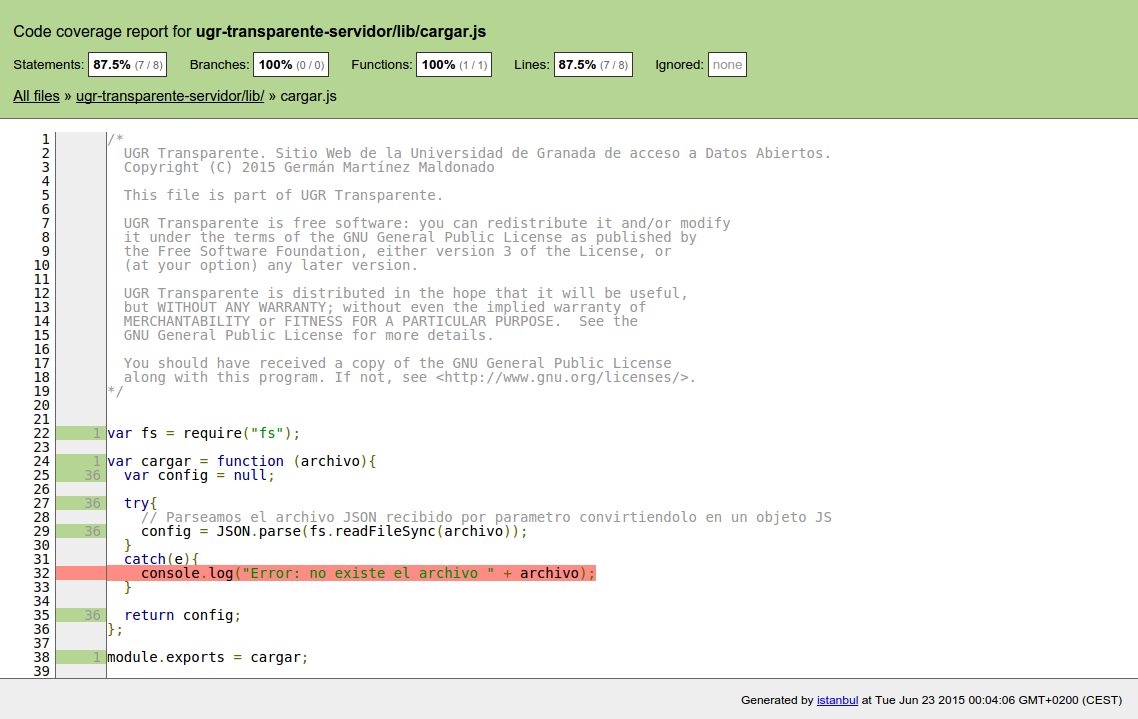
\includegraphics[width=1\textwidth]{../images/test_cobertura_03.png}
		\caption{}
		\label{fig:test_cobertura_03}
	\end{center}
\end{figure}

\section{Integración continua}

\begin{figure}[!ht]
	\begin{center}
		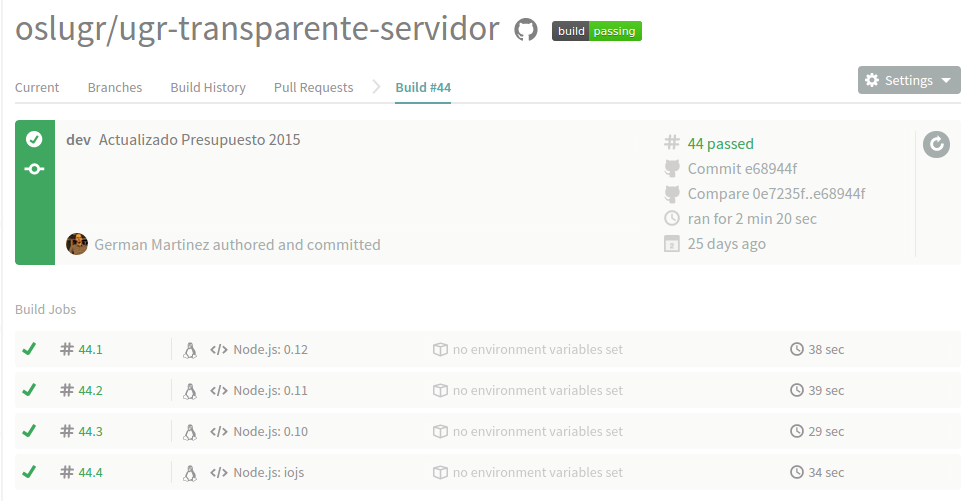
\includegraphics[width=1\textwidth]{../images/integracion_continua_01.png}
		\caption{}
		\label{fig:integracion_continua_01}
	\end{center}
\end{figure}

\begin{figure}[!ht]
	\begin{center}
		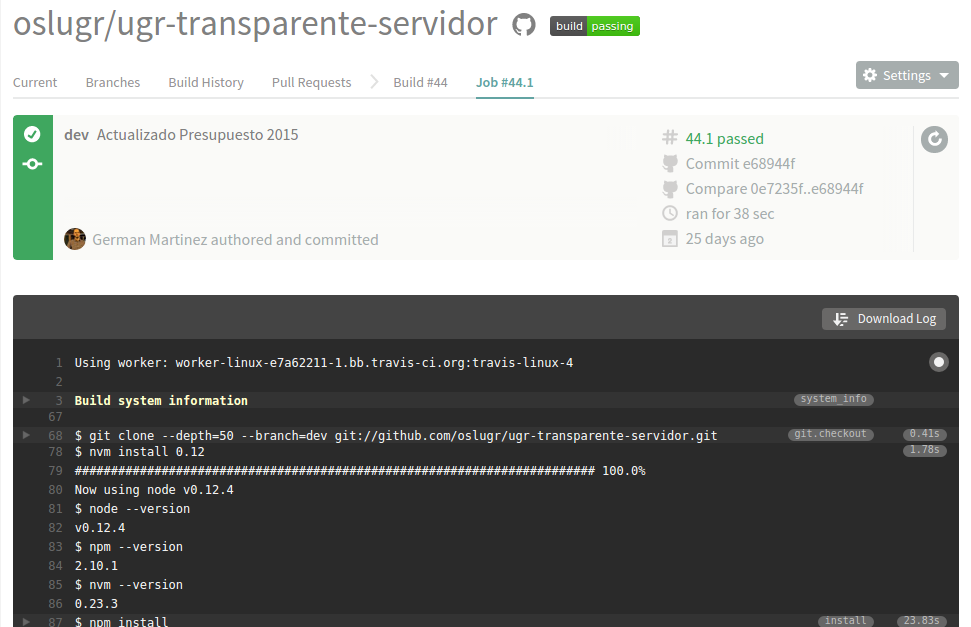
\includegraphics[width=1\textwidth]{../images/integracion_continua_02.png}
		\caption{}
		\label{fig:integracion_continua_02}
	\end{center}
\end{figure}

\begin{figure}[!ht]
	\begin{center}
		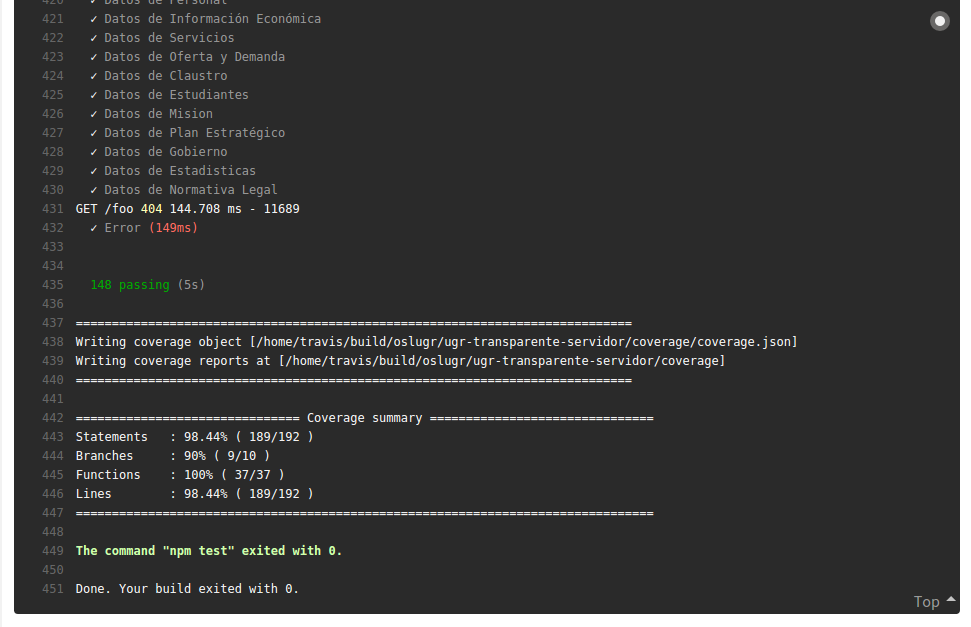
\includegraphics[width=1\textwidth]{../images/integracion_continua_03.png}
		\caption{}
		\label{fig:integracion_continua_03}
	\end{center}
\end{figure}

\newpage \
\newpage \
\newpage \
\newpage \
\newpage \
\section{Prueba de carga}

\subsection{Métricas y parámetros que afectan al rendimiento}

Para comparar las prestaciones de la aplicación debemos tener en cuenta los siguientes criterios:

\begin{itemize}
	\item El objetivo de esta prueba es medir las prestaciones del servidor generado por {\tt Express} para dar servicio a la aplicación del portal de transparencia bajo unas condiciones que nos aporte un análisis neutro del rendimiento del mismo.
	\item La herramienta que se usará para realizar estás mediciones es {\tt ApacheBench}.
	\item Los parámetros que se considerarán los parámetros usados en la herramienta: el número de peticiones que se realizan al servidor y el nivel de concurrencia con el que se realizan las peticiones.
	\item Los valores de estos parámetros irán modificándose para tener unos resultados más completos ante las diferentes cargas de trabajo que soportará el servidor.
\end{itemize}

El hardware y el software del sistema serán los siguientes:

\begin{itemize}
	\item \textbf{Hardware}:
	\begin{itemize}
		\item Procesador: Intel Pentium Dual CPU E2180 @ 2.00GHz
		\item Placa base: MSI MS-7255
		\item Chipset: VIA P4M900
		\item Memoria: 3GB (2+1 DIMM DDR2)
		\item Disco: Maxtor 6Y160P0 160GB 7200RPM
		\item Tarjeta gráfica: ATI Radeon X300SE 325MHz 128MB
		\item Red: Realtek RTL8100C 100Mbps
	\end{itemize}
	\item \textbf{Software}:
	\begin{itemize}
		\item Sistema operativo: Ubuntu 14.04.1 LTS i686 GNU/Linux
		\item Kernel: Linux 3.13.0-35-generic
		\item Sistema de archivos: ext4
	\end{itemize}
\end{itemize}

\subsection{Técnicas de evaluación, carga de trabajo y diseño de experimentos}

Para evaluar el rendimiento de la aplicación vamos a realizar benchmark hacia la aplicación en ejecución para poder realizar una evaluación sobre su comportamiento bajo diferentes cargas de trabajo. El programa con el que vamos hacer las pruebas es el ya mencionado {\tt ApacheBench}.
{\tt ApacheBench} es un aplicación en modo terminal que permite realizar de forma sencilla pruebas de rendimiento a cualquier servidor, sea cual sea el lenguaje en el que esté realizado. 

\bigskip
Según la información de registros de acceso del servidor en los últimos \textbf{6 meses} el número de peticiones de páginas del portal ha sido de \textbf{2.388 peticiones}, lo que sería aproximadamente \textbf{13 peticiones/día}. Para realizar los diferentes tests se realizará un \textbf{número de conexiones} variables al servidor (\textbf{30, 50 y 100}) con diferentes \textbf{niveles de concurrencia} en función del total de conexiones (\textbf{25\%, 50\% y 75\%}). Los números de conexiones para las prueba han sido elegidos para evaluar como se comportaría el servidor ante un gran aumento de actividad en el mismo en línea con el nivel de conexiones que se producen en la actualidad.

\bigskip
De entre las peticiones al portal, la página que ha recibido un mayor número de peticiones es la página de \textbf{Personal}, por lo que el experimento a realizar consistirá en realizar peticiones de la página de \textbf{Personal} a la aplicación. Este experimente nos permitirá comprobar como se comportará la aplicación en diferentes situaciones cono diferentes niveles de carga y la repercusión en su rendimiento ante estás diferentes pruebas, viendo por ejemplo si fuera necesario buscar una forma de balancear la carga del servidor. 

\bigskip
En total el experimento constará de 9 pruebas, y a su vez cada una de estas pruebas se repetirá 10 veces consecutivas para así asegurarnos que los resultados son legítimos y no producto de sucesos fortuitos. Los resultados mostrados serán la media de esas 10 ejecuciones y su desviación estándar, que nos permitirá saber como de válidos podemos considerar los valores medios obtenidos. Estos valores promedios se introducirán en un gráfico para comparar los cambios que se producen con diferentes números de conexiones y mismos porcentaje de concurrencia.

\bigskip
Las variables respuestas a tener en cuenta para el estudio serán:

\begin{itemize}
	\item Tiempo de ejecución.
	\item Solicitudes por segundo.
	\item Tiempo por solicitud concurrente.
	\item Velocidad de transferencia.
\end{itemize}

\bigskip
El único factor a considerar para el experimento será, como hemos dicho, las respuestas del servidor de la aplicación desarrollada del portal de transparencia {\tt UGR Transparente}. Cuando se disponga de los resultados de todas las pruebas, se procederá a analizar e interpretar los resultados.

\subsection{Presentación de los resultados}

Enumeración de las pruebas a realizar en el experimento:

\begin{itemize}
	\item \textbf{Prueba 1}: 30 solicitudes, concurrencia del 25\% (8).
	\item \textbf{Prueba 2}: 30 solicitudes, concurrencia del 50\% (15).
	\item \textbf{Prueba 3}: 30 solicitudes, concurrencia del 75\% (23).
	\item \textbf{Prueba 4}: 50 solicitudes, concurrencia del 25\% (13).
	\item \textbf{Prueba 5}: 50 solicitudes, concurrencia del 50\% (25).
	\item \textbf{Prueba 6}: 50 solicitudes, concurrencia del 75\% (38).
	\item \textbf{Prueba 7}: 100 solicitudes, concurrencia del 25\% (25).
	\item \textbf{Prueba 8}: 100 solicitudes, concurrencia del 50\% (50).
	\item \textbf{Prueba 9}: 100 solicitudes, concurrencia del 75\% (75).
\end{itemize}

\newpage
\subsubsection{Tiempo de ejecución}
\begin{table}[!ht]
	\begin{center}
		\begin{tabular}{|c|c|c|c|}
			\hline
			\multicolumn{4}{|c|}{{\bf Tiempo de ejecución}}                                                           \\ \hline
			{\bf N.º conexiones} & {\bf Concurrencia (\%)} & {\bf Segundos} & {\bf Desviación} \\ \hline
			{\it 30}                   & {\it 25}                  & 8,823              & 0,199                     \\ \hline
			{\it 30}                   & {\it 50}                  & 7,552              & 0,214                     \\ \hline
			{\it 30}                   & {\it 75}                  & 6,827              & 0,970                     \\ \hline
			{\it 50}                   & {\it 25}                  & 10,215             & 0,248                     \\ \hline
			{\it 50}                   & {\it 50}                  & 12,506             & 0,299                     \\ \hline
			{\it 50}                   & {\it 75}                  & 13,959             & 0,217                     \\ \hline
			{\it 100}                  & {\it 25}                  & 26,966             & 1,781                     \\ \hline
			{\it 100}                  & {\it 50}                  & 22,850             & 3,845                     \\ \hline
			{\it 100}                  & {\it 75}                  & 24,473             & 3,845                     \\ \hline
		\end{tabular}
		\caption{Resultados de tiempo de ejecución}
		\label{table:rte}
	\end{center}
\end{table}

\begin{figure}[!ht]
	\begin{center}
		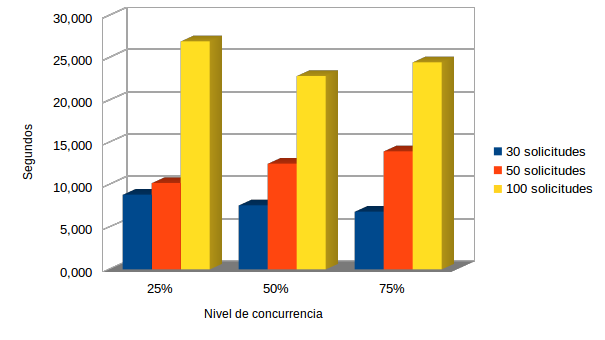
\includegraphics[width=1\textwidth]{../images/gra_te.png}
		\caption{Gráfico de tiempo de ejecución}
		\label{fig:gra_te}
	\end{center}
\end{figure}

\newpage
\subsubsection{Solicitudes por segundo}
\begin{table}[!ht]
	\begin{center}
		\begin{tabular}{|c|c|c|c|}
			\hline
			\multicolumn{4}{|c|}{{\bf Solicitudes por segundo}}                                                   \\ \hline
			{\bf N.º de conexiones} & {\bf Concurrencia (\%)} & {\bf Solicitudes/s} & {\bf Desviación} \\ \hline
			{\it 30}                & {\it 25}                & 3,402                          & 0,078            \\ \hline
			{\it 30}                & {\it 50}                & 3,976                          & 0,113            \\ \hline
			{\it 30}                & {\it 75}                & 4,470                          & 0,531            \\ \hline
			{\it 50}                & {\it 25}                & 4,898                          & 0,118            \\ \hline
			{\it 50}                & {\it 50}                & 4,000                          & 0,095            \\ \hline
			{\it 50}                & {\it 75}                & 3,583                          & 0,056            \\ \hline
			{\it 100}               & {\it 25}                & 3,728                          & 0,292            \\ \hline
			{\it 100}               & {\it 50}                & 4,496                          & 0,708            \\ \hline
			{\it 100}               & {\it 75}                & 4,197                          & 0,703            \\ \hline
		\end{tabular}
		\caption{Resultados de solicitudes por segundo}
		\label{table:rss}
	\end{center}
\end{table}

\begin{figure}[!ht]
	\begin{center}
		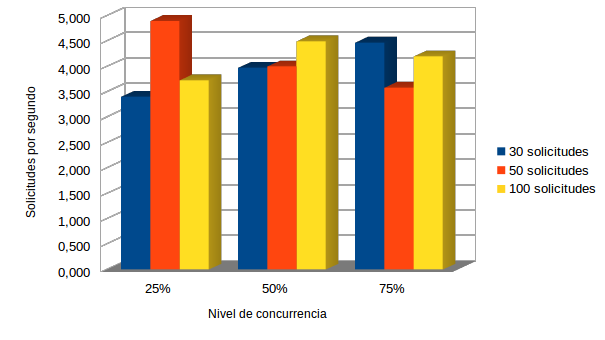
\includegraphics[width=1\textwidth]{../images/gra_sps.png}
		\caption{Gráfico de solicitudes por segundo}
		\label{fig:gra_sps}
	\end{center}
\end{figure}

\newpage
\subsubsection{Tiempo por solicitud concurrente}
\begin{table}[!ht]
	\begin{center}
		\begin{tabular}{|c|c|c|c|}
			\hline
			\multicolumn{4}{|c|}{{\bf Tiempo por solicitud concurrente}}                               \\ \hline
			{\bf N.º de conexiones} & {\bf Concurrencia (\%)} & {\bf Promedio (ms)} & {\bf Desviación} \\ \hline
			{\it 30}                & {\it 25}                & 294,087             & 6,645            \\ \hline
			{\it 30}                & {\it 50}                & 251,733             & 7,129            \\ \hline
			{\it 30}                & {\it 75}                & 227,563             & 32,347           \\ \hline
			{\it 50}                & {\it 25}                & 204,296             & 4,959            \\ \hline
			{\it 50}                & {\it 50}                & 250,128             & 5,990            \\ \hline
			{\it 50}                & {\it 75}                & 279,178             & 4,346            \\ \hline
			{\it 100}               & {\it 25}                & 269,658             & 17,811           \\ \hline
			{\it 100}               & {\it 50}                & 228,497             & 38,451           \\ \hline
			{\it 100}               & {\it 75}                & 244,729             & 38,449           \\ \hline
		\end{tabular}
		\caption{Resultados de tiempo por solicitud concurrente}
		\label{table:rtsc}
	\end{center}
\end{table}

\begin{figure}[!ht]
	\begin{center}
		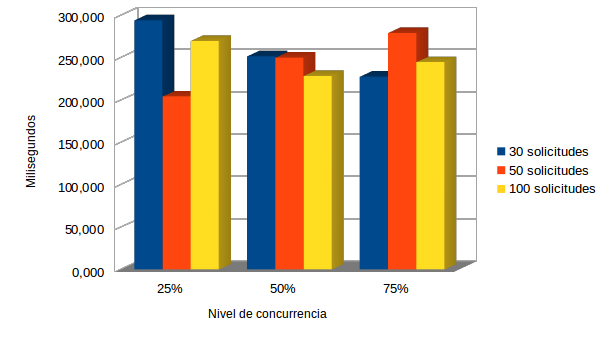
\includegraphics[width=1\textwidth]{../images/gra_tsc.png}
		\caption{Gráfico de tiempo por solicitud concurrente}
		\label{fig:gra_tsc}
	\end{center}
\end{figure}

\newpage
\subsubsection{Velocidad de transparencia}
\begin{table}[!ht]
	\begin{center}
		\begin{tabular}{|c|c|c|c|}
			\hline
			\multicolumn{4}{|c|}{{\bf Velocidad de transferencia}}                            \\ \hline
			{\bf N.º de conexiones} & {\bf Concurrencia (\%)} & {\bf KB/s} & {\bf Desviación} \\ \hline
			{\it 30}                & {\it 25}                & 747,735    & 17,116           \\ \hline
			{\it 30}                & {\it 50}                & 873,789    & 24,798           \\ \hline
			{\it 30}                & {\it 75}                & 982,389    & 116,778          \\ \hline
			{\it 50}                & {\it 25}                & 645,866    & 15,498           \\ \hline
			{\it 50}                & {\it 50}                & 527,515    & 12,561           \\ \hline
			{\it 50}                & {\it 75}                & 472,469    & 7,339            \\ \hline
			{\it 100}               & {\it 25}                & 245,783    & 19,227           \\ \hline
			{\it 100}               & {\it 50}                & 296,416    & 46,684           \\ \hline
			{\it 100}               & {\it 75}                & 276,707    & 46,384           \\ \hline
		\end{tabular}
		\caption{Resultados de velocidad de transferencia}
		\label{table:rvt}
	\end{center}
\end{table}

\begin{figure}[!ht]
	\begin{center}
		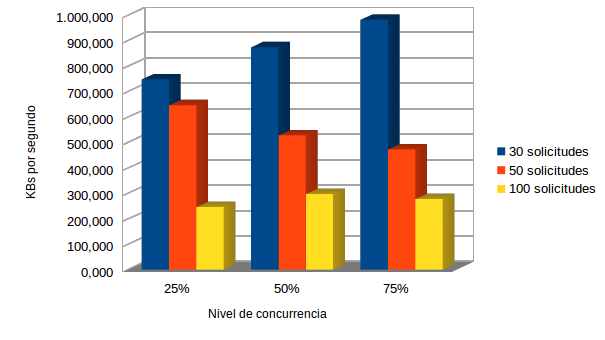
\includegraphics[width=1\textwidth]{../images/gra_vt.png}
		\caption{Gráfico de velocidad de transferencia}
		\label{fig:gra_te}
	\end{center}
\end{figure}

\newpage
\subsection{Análisis e interpretación de los resultados}

\subsubsection{Tiempo de ejecución}
\begin{itemize}
	\item Para un número de 30 conexiones (poco más de la media de conexiones diarias al portal) la concurrencia no afecta al tiempo de respuesta de la aplicación.
	\item Cuando el número de conexiones aumenta hasta 50, vemos como en este el nivel de concurrencia sí empieza a afectar al tiempo de respuesta de la aplicación de forma negativa.
	\item En la última prueba con un número de conexiones bastante más elevado, vemos en los tiempos de ejecución que el comportamiento es más aleatorio. Si nos fijamos en las desviaciones estás han crecido bastante en comparación con las pruebas anteriores, por lo que aparentemente la aplicación empieza a soportar cierta sobrecarga.
\end{itemize}

\subsubsection{Solicitudes por segundo}
\begin{itemize}
	\item En relación directa con los resultados descritos en el apartado anterior vemos que para 30 conexiones, al igual que el tiempo de respuesta bajaba según el nivel de concurrencia, ahora el número de solicitudes respondidas por segundo aumentan; el comportamiento que cabría esperar.
	\item En el caso de 50 conexiones, de igual forma, cuando el nivel de concurrencia sube, el número de solicitudes respondidas baja.
	\item Para la prueba de 100 conexiones volvemos a tener una situación similar a la anterior, donde aunque en esta caso las desviaciones no son tan altas, no se puede concretar una tendencia en el rendimiento de la aplicación.
\end{itemize}

\subsubsection{Tiempo por solicitud concurrente}
\begin{itemize}
	\item Se produce la misma situación, para 30 conexiones el tiempo necesario para resolver una solicitud recurrente va disminuyendo según aumenta la concurrencia en las conexiones. A destacar que en esta prueba el valor de la desviación crece en gran cantidad, por lo que aunque se puede encontrar una tendencia general de mejor en el rendimiento los tiempos para resolver las solicitudes no son tan homogéneos.
	\item En el caso de las 50 conexiones también se produce la misma situación a las pruebas anteriores: según aumenta la concurrencia aumenta el tiempo necesario para responder una solicitud concurrente, lo que indica que el rendimiento ha bajado.
	\item De igual forma, para 100 conexiones volvemos a encontrar sin un patrón claro de comportamiento, pero si podemos destacar que las desviaciones son enormes.
\end{itemize}

\subsubsection{Velocidad de transferencia}
\begin{itemize}
	\item Mismo patrón para la prueba con 30 conexiones. Habíamos visto que según aumenta la concurrencia, disminuye el tiempo de ejecución y aumentan el número de solicitudes por segundo respondidas o lo que es lo mismo, aumenta el rendimiento; así que como podríamos intuir y con estos datos comprobar, también aumenta la cantidad de información transferida. Nos encontramos en algunos casos con desviaciones enormes, pero eso podemos atribuirlo a la propia naturaleza inestable de las conexiones de red.
	\item Como se ha venido produciendo, en el caso de la prueba con 50 conexiones el rendimiento ha ido bajando según ha ido aumentando el porcentaje de concurrencia; esto también se produce en este caso: según aumentaba la concurrencia, disminuía la velocidad de transferencia.
	\item Por último, en la prueba con 100 conexiones esta es la prueba que ha tenido resultados más igualados (y además muy bajos en comparación) entre los diferentes niveles de concurrencia, lo que nos vuelve a hacer suponer que el servidor está sobrecargado.
\end{itemize}

\subsection{Conclusiones sobre los resultados}